\lstset{
	basicstyle=\ttfamily,
	numbers=left,
	numberstyle=\color{gray},
	tabsize=2,
	language=C,
	morekeywords={exec,sql}
}
\begin{document}
\lecture{Implementierung von Datenbanksystemen}{IDB}
\title{Übungsblatt~9}
\subtitle{Speicherung}
\maketitle

\section*{Lernziele}

\begin{itemize}
  \item Erstellung und algebraische Optimierung von Ausführungsplänen mit Sichten
  \item Optimierung in der Praxis
\end{itemize}

\section*{Literatur}

\HaerderNintyNine{11, 12}

\ElmasriSeventh{18, 19}

\GarciaMolinaSecond{8, 15, 16}

\NeumannFifteen


\section{Fragen zur Vorlesung}

\begin{enumerate}[a)]
	\item Was ist die Aufgabe der Anfrageverarbeitung?

	\begin{solution}
	Abbildung von mengenorientierten Operationen auf effiziente satzorientierte Operationen.
	D.\,h.\ von oben kommen nun keine Satzoperationen mehr, sondern mengenorientierte (Relationenalgebra, SQL).
	Das verringert oft den Programmieraufwand (Beispiel: Mitarbeiter und Abteilungen, VL 10-22).
	Außerdem ist es einfacher zu optimieren.
	Insbesondere muss bei Änderungen an Kardinalitäten etc.\ nicht die Programmstruktur geändert werden.
	Das macht der Optimierer für uns.
	\end{solution}

	\item Aus welchen Schritten besteht sie?

	\begin{note}
	Bild an die Tafel.\\
	Oracle macht das übrigens so 	\url{https://docs.oracle.com/database/121/TGSQL/tgsql_sqlproc.htm\#TGSQL175}
	\end{note}
	\beamertxt{\pagebreak}

	\begin{solution}
	Siehe Folien~\Anfrageverarbeitung.

	Härder:
		Parser macht lexikalische und syntaktische Analyse.
		Semantische Analyse wird bereits mit der Interndarstellung gemacht.
		Das sind Namensauflösung und Typumwandlung.
		Zugriffs- und Integritätskontrolle sind eine Erweiterung der semantischen Analyse.
		"`Standardisierung und Vereinfachung"' und "`Restrukturierung und Transformation"' sind gemeinsam die Optimierung.
	\end{solution}

	\item Angenommen eine Anfrage wird mit gleichen Parametern erneut ausgeführt: Welche Schritte könnten unter welchen Bedingungen eingespart werden?

	\begin{solution}
	Das ist schwieriger, als man denkt:
\begin{itemize}
	\item Sollten sich die Daten nicht geändert haben, könnte man das selbe Ergebnis zurückgeben.
	\item Wenn sich die Daten nur leicht ändern, müsste man nur die Ausführung erneut durchführen, da sich ein anderes Ergebnis ergibt.
	\item Ändern sich die Daten stark, so muss auch die Optimierung erneut durchgeführt werden.
	\item Ändern die Berechtigungen, so muss die Zugriffskontrolle erneut durchgeführt werden.
\end{itemize}
	Rein theoretisch kann man diese Fälle feststellen (Jedes Grant/Revoke prüfen; Statistiken für den Optimierer werden nur explizit geändert, dann kann man prüfen.),
	jedoch wird in der Praxis mit wenigen Ausnahmen einfach die gesamte Anfrageverarbeitung erneut durchgeführt.
	Eine Ausnahme bilden explizit gespeicherte Prozeduren und Funktionen (z.b. PL/SQL).
	\end{solution}

	\item Nun mit unterschiedlichen Parametern.

	\begin{solution}
	Zusätzlich zu den obigen Schritten muss nur die Typkonversion erneut durchgeführt werden.
	Sinnvoll kann zusätzlich eine erneute Optimierung sein ($\mathrm{Wert} > 10$; $\mathrm{Wert} > 1000000$).
	\end{solution}
\end{enumerate}
\begin{beamerText}
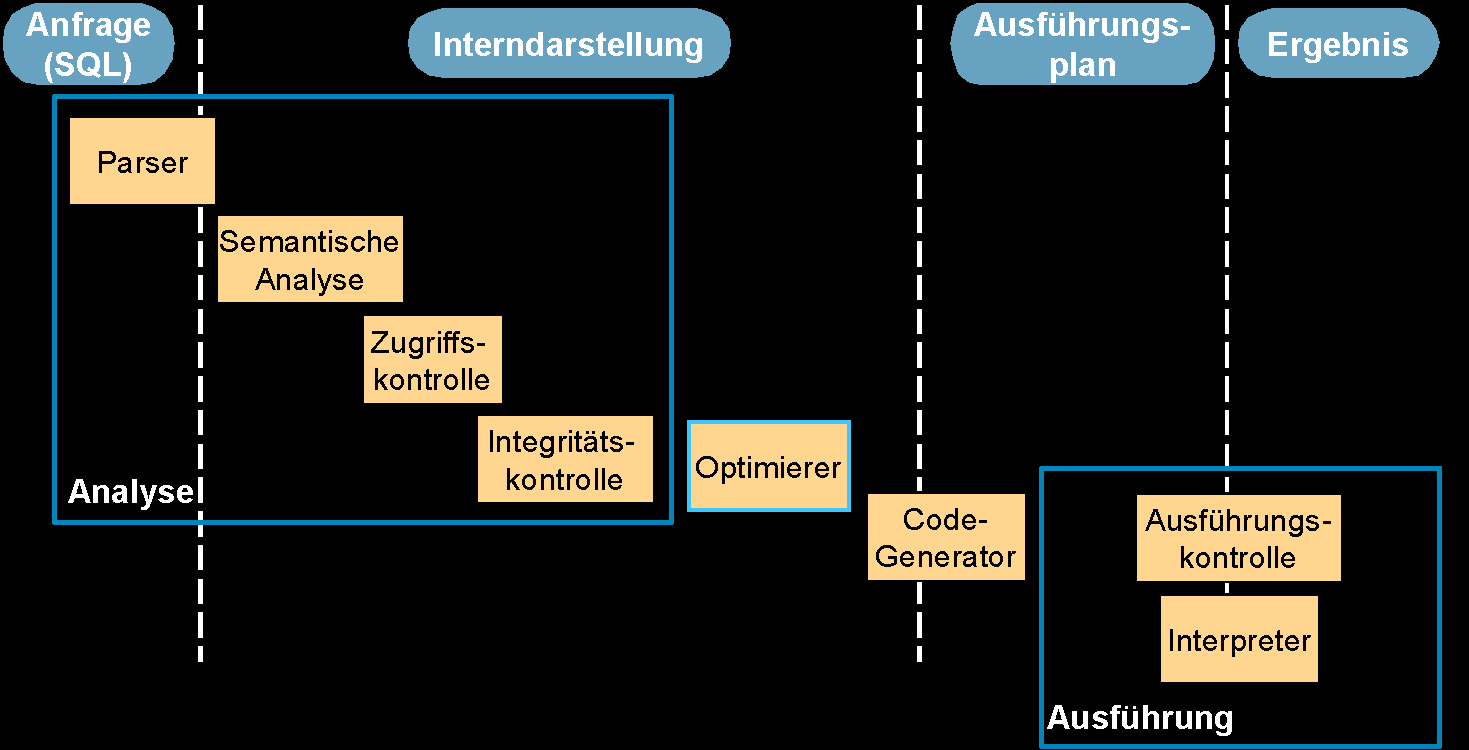
\includegraphics[width=1\linewidth]{Pictures/U10-Beamer-Anfrageverarbeitung}
\pagebreak
\end{beamerText}


\beamertxt{\pagebreak}
\section{Speicherungsstrukturen in Sätzen}

Betrachten Sie die folgende Relation "`Kunden"':

\texttt{
\begin{tabbing}
----------------------------- \= \kill
Kundennr \> NUMBER(6) \\
Name \> VARCHAR2(120) \\
PLZ \> NUMBER(5) \\
Ort \> VARCHAR2(120) \\
LetzterEinkauf \> DATE
\end{tabbing}
}

Das verwendete DBMS orientiert sich an Oracle. Die Angabe \texttt{NUMBER(6)} bedeutet, dass positive und negative Zahlen mit maximal 6~Dezimalstellen gespeichert werden können. Bei der Speicherung numerischer Daten werden ein Byte für den Exponenten und maximal 20~Byte für die Mantisse benutzt. Jeweils zwei Ziffern belegen ein Byte der Mantisse. Eine negative Zahl wird durch eine zusätzliche Ziffer dargestellt, die nicht im Bereich von [0..9] liegt. Ein Datumsfeld umfasst stets 7~Byte. Die Längenangabe in der Schemadefinition erfolgt bei \texttt{VARCHAR2} standardmäßig in Byte. Wir verwenden eine Zeichenkodierung, bei der je Zeichen 2~Byte benötigt werden (z.\,B.\ UTF-16). Eine Längenangabe soll einheitlich 4~Byte lang sein.

\begin{solution}
In Oracle berechnet sich die Feldlänge numerischer Daten wie folgt:

\[\left\lceil\frac{p + s}{2}\right\rceil + 1 \, \mathrm{[Bytes]}\]

mit $p =$ Anzahl der Dezimalstellen des zu speichernden Datums und $s = 0$ für die Speicherung einer positiven, $s = 1$ für die Speicherung einer negativen Zahl. Man beachte hierbei, dass die Feldlänge jedes Eintrags unterschiedlich sein kann.

Hierdurch ergibt sich für \texttt{NUMBER(6)} die Maximallänge \[\left\lceil\frac{\texttt{Länge} + \texttt{mögliches Signum}}{2}\right\rceil + \texttt{Länge Exponent} = \left\lceil\frac{6 + 1}{2}\right\rceil + 1 = 5 \, \mathrm{[Bytes]}\]

\paragraph{Beispielcodierungen:}
Das Minuszeichen wird in diesem Beispiel as 0xF dargestellt, beim negativen Exponenten ist das größte Bit gesetzt.\\
\begin{tabular}{lllp{3.5cm}l}
	\hline\hline
	Zahl    & Speicherdarstellung    & hexadezimal   & binär                                   & Feldlänge \\ \hline\hline
	20.000  & $0,\!2\cdot10^6$       & 0x20 0x06     & 0010 0000 0000 0110                     & 2         \\ \hline
	-20.000 & $-0,\!2\cdot10^{6}$    & 0xF2 0x06     & 1111 0010 0000 0110                     & 2         \\ \hline
	12.345  & $0,\!12345\cdot10^{6}$ & 0x123450 0x06 & 0001 0010 0011 0100 0101 0000 0000 0110 & 4         \\ \hline
\end{tabular}

\end{solution}
\begin{note}
Jup, oracle macht das wirklich so.. (Oder so ähnlich)
\url{https://docs.oracle.com/cd/B19306\_01/server.102/b14220/datatype.htm\#sthref3818}
\end{note}
\beamertxt{\pagebreak}

\begin{enumerate}[a)]
	\item \label{Speicherungsstrukturen_1} Fügen Sie in die Relation "`Kunden"' die folgenden beiden Datensätze ein und geben Sie zu jedem Datensatz die Speicherungsstruktur wie in der Vorlesung vorgestellt an. Gehen Sie von Feldern fester, d.\,h.\ maximaler Länge aus. Wie viele Bytes umfasst jeder Satz?

	\texttt{1, Müller, 91058, Erlangen, 2010-04-27 9:57:21}

	\texttt{4711, Huber, 90403, Nürnberg, 2010-01-24 11:17:33}

	\begin{solution}
	\begin{tabular}{lllll}
		\hline\hline
		\textbf{Feldname} & \textbf{Datentyp} & \textbf{Pos.} & \textbf{Feldinhalt}                & \textbf{Feldlän.} \\ \hline\hline
		Gesamtlänge       & Längenabgabe      & 0             & 260 (alt. 293)                     & 4                 \\ \hline
		Kundennr.         & NUMBER(6)         & 1             & 1                                  & 5  (alt. 21)      \\ \hline
		Name              & VARCHAR2(120)     & 2             & Müller                             & 120               \\ \hline
		PLZ               & NUMBER(5)         & 3             & 91058                              & 4 (alt. 21)       \\ \hline
		Ort               & VARCHAR2(120)     & 4             & Erlangen                           & 120               \\ \hline
		Letzter Einkauf   & DATE              & 5             & \footnotesize{2010-04-27 09:57:21} & 7                 \\ \hline
	\end{tabular}

    Beim zweiten Datensatz ändert sich lediglich die Spalte "`Feldinhalt"'.

	Diskussion:
Die Gesamtlänge könnte man hier weglassen und stattdessen aus dem Metadatenkatalog nehmen, sie ist ja für alle Sätze gleich. Wir halten uns an die Vorlesungsfolien, die diesen Wert in den Sätzen ablegen.
Ein \texttt{NUMBER(6)} lässt sich immer in 5~Bytes speichern (Nach obiger Formel: 1 Exponent, 3 Mantisse, 1 Vorzeichen).

\underline{Hinweis zu (alt. 21):}
Laut Oracle hat zwar ein \texttt{NUMBER(N)} 1 Byte für den Exponenten und maximal 20 für die Mantisse und damit 21 Byte.
Jedoch wird die Länge eines \texttt{NUMBER(N)} mithilfe der obigen Formel berechnet.


Außerdem muss man herausfinden können, wie viele Daten in Wirklichkeit in den VARCHAR-Feldern stehen. Das könnte man z.\,B.\ durch Null-Terminierung erreichen. Wenn man dann den vorhandenen Platz vollständig ausfüllt, dann kann man aber kein Terminierungszeichen mehr unterbringen. Das lässt sich dadurch lösen, dass man bis zum Null-Character liest, höchstens jedoch die Maximalzahl an Bytes.
	\end{solution}

	\item \label{Speicherungsstrukturen_2} Fügen Sie die beiden Datensätze von Teilaufgabe \ref{Speicherungsstrukturen_1}) ein und verwenden Sie Felder variabler Länge.

	\begin{solution}
	\begin{tabular}{lllll}
		\hline\hline
		\textbf{Feldname} & \textbf{Datentyp} & \textbf{Pos.} & \textbf{Feldinhalt}                & \textbf{Feldlän.} \\ \hline\hline
		Gesamtlänge       & Längenabgabe      & 0             & 61                                 & 4                 \\ \hline
		Länge Kundennr.   & Längenangabe      & 1             & 2                                  & 4                 \\ \hline
		Kundennr.         & NUMBER(6)         & 2             & 1                                  & 2                 \\ \hline
		Länge Name        & Längenangabe      & 3             & 12                                 & 4                 \\ \hline
		Name              & VARCHAR2(120)     & 4             & Müller                             & 12                \\ \hline
		Länge PLZ         & Längenangabe      & 5             & 4                                  & 4                 \\ \hline
		PLZ               & NUMBER(5)         & 6             & 91058                              & 4                 \\ \hline
		Länge Ort         & Längenangabe      & 7             & 16                                 & 4                 \\ \hline
		Ort               & VARCHAR2(120)     & 8             & Erlangen                           & 16                \\ \hline
		Letzter Einkauf   & DATE              & 9             & \footnotesize{2010-04-27 09:57:21} & 7                 \\ \hline
	\end{tabular}
	
	\begin{tabular}{lllll}
		\hline\hline
		\textbf{Feldname} & \textbf{Datentyp} & \textbf{Pos.} & \textbf{Feldinhalt}                & \textbf{Feldlän.} \\ \hline\hline
		Gesamtlänge       & Längenabgabe      & 0             & 60                                 & 4                 \\ \hline
		Länge Kundennr.   & Längenangabe      & 1             & 3                                  & 4                 \\ \hline
		Kundennr.         & NUMBER(6)         & 2             & 4711                               & 3                 \\ \hline
		Länge Name        & Längenangabe      & 3             & 10                                 & 4                 \\ \hline
		Name              & VARCHAR2(120)     & 4             & Huber                              & 10                \\ \hline
		Länge PLZ         & Längenangabe      & 5             & 4                                  & 4                 \\ \hline
		PLZ               & NUMBER(5)         & 6             & 90403                              & 4                 \\ \hline
		Länge Ort         & Längenangabe      & 7             & 16                                 & 4                 \\ \hline
		Ort               & VARCHAR2(120)     & 8             & Nürnberg                           & 16                \\ \hline
		Letzter Einkauf   & DATE              & 9             & \footnotesize{2010-01-24 11:17:33} & 7                 \\ \hline
	\end{tabular}

Hier kann man wieder diskutieren, ob die Längenfelder notwendig sind.
Die Gesamtlänge wird man wohl speichern (obwohl man sie auch aus der blockinternen Zeigerliste, siehe Übung zu TIDs, lesen könnte).
Auch um die Feldlängen kommt man nicht herum.
Achtung: Feldlängen speichert man nur für die Felder variabler Größe.
	\end{solution}

	\item Fügen Sie die Datensätze von Teilaufgabe \ref{Speicherungsstrukturen_1}) unter Verwendung von Zeigern ein. Ein Zeiger soll die Länge 4 besitzen.

	\begin{solution}
	{\small
	\begin{tabular}{p{2.8cm}lllll}
		\hline\hline
		\textbf{Feldname}         & \textbf{Datentyp} & \textbf{Pos.} & \textbf{Pos. (Bytes)} & \textbf{Feldinhalt}                & \textbf{Feldlän.} \\ \hline\hline
		Gesamtlänge               & Längenabgabe      & 0             & 0                     & 81                                 & 4                 \\ \hline
		Länge Fester Strukturteil & Längenangabe      & 1             & 4                     & 31                                 & 4                 \\ \hline
		Zeiger Kundennr.          & Zeiger            & 2             & 8                     & Pos. 7 (Byte 31)                   & 4                 \\ \hline
		Zeiger Name               & Zeiger            & 3             & 12                    & Pos. 9 (Byte 37)                   & 4                 \\ \hline
		Zeiger PLZ                & Zeiger            & 4             & 16                    & Pos. 11 (Byte 53)                  & 4                 \\ \hline
		Zeiger Ort                & Zeiger            & 5             & 20                    & Pos. 13 (Byte 61)                  & 4                 \\ \hline
		Letzter Einkauf           & DATE              & 6             & 24                    & \footnotesize{2010-04-27 09:57:21} & 7                 \\ \hline
		Länge Kundennr.           & Längenangabe      & 7             & 31                    & 2                                  & 4                 \\ \hline
		Kundennr.                 & NUMBER(6)         & 8             & 35                    & 1                                  & 2                 \\ \hline
		Länge Name                & Längenangabe      & 9             & 37                    & 12                                 & 4                 \\ \hline
		Name                      & VARCHAR2(120)     & 10            & 41                    & Müller                             & 12                \\ \hline
		Länge PLZ                 & Längenangabe      & 11            & 53                    & 4                                  & 4                 \\ \hline
		PLZ                       & NUMBER(5)         & 12            & 57                    & 91058                              & 4                 \\ \hline
		Länge Ort                 & Längenangabe      & 13            & 61                    & 16                                 & 4                 \\ \hline
		Ort                       & VARCHAR2(120)     & 14            & 65                    & Erlangen                           & 16                \\ \hline
	\end{tabular}}

{\small
	\begin{tabular}{p{2.8cm}lllll}
		\hline\hline
		\textbf{Feldname}         & \textbf{Datentyp} & \textbf{Pos.} & \textbf{Pos. (Bytes)} & \textbf{Feldinhalt}                & \textbf{Feldlän.} \\ \hline\hline
		Gesamtlänge               & Längenabgabe      & 0             & 0                     & 80                                 & 4                 \\ \hline
		Länge Fester Strukturteil & Längenangabe      & 1             & 4                     & 31                                 & 4                 \\ \hline
		Zeiger Kundennr.          & Zeiger            & 2             & 8                     & Pos. 7 (Byte 31)                   & 4                 \\ \hline
		Zeiger Name               & Zeiger            & 3             & 12                    & Pos. 9 (Byte 38)                   & 4                 \\ \hline
		Zeiger PLZ                & Zeiger            & 4             & 16                    & Pos. 11 (Byte 52)                  & 4                 \\ \hline
		Zeiger Ort                & Zeiger            & 5             & 20                    & Pos. 13 (Byte 60)                  & 4                 \\ \hline
		Letzter Einkauf           & DATE              & 6             & 24                    & \footnotesize{2010-01-24 11:17:33} & 7                 \\ \hline
		Länge Kundennr.           & Längenangabe      & 7             & 31                    & 3                                  & 4                 \\ \hline
		Kundennr.                 & NUMBER(6)         & 8             & 35                    & 4711                               & 3                 \\ \hline
		Länge Name                & Längenangabe      & 9             & 38                    & 10                                 & 4                 \\ \hline
		Name                      & VARCHAR2(120)     & 10            & 42                    & Huber                              & 10                \\ \hline
		Länge PLZ                 & Längenangabe      & 11            & 52                    & 4                                  & 4                 \\ \hline
		PLZ                       & NUMBER(5)         & 12            & 56                    & 90403                              & 4                 \\ \hline
		Länge Ort                 & Längenangabe      & 13            & 60                    & 16                                 & 4                 \\ \hline
		Ort                       & VARCHAR2(120)     & 14            & 64                    & Nürnberg                           & 16                \\ \hline
	\end{tabular}}

	Auch hier: Diskussion über Längenfelder.
Gesamtlänge siehe \ref{Speicherungsstrukturen_2}).
Länge für einzelne Felder: Die könnte man jetzt dadurch berechnen, dass man den aktuellen Zeiger vom nächsten abzieht. Das wird aber komplexer, wenn zwischen zwei Feldern variabler Länge solche mit fester Länge liegen.
	\end{solution}

\end{enumerate}

\begin{beamerText}
\pagebreak
{\small
	\texttt{1, Müller, 91058, Erlangen, 2010-04-27 9:57:21}\\
	\texttt{4711, Huber, 90403, Nürnberg, 2010-01-24 11:17:33}
}\\
\begin{minipage}{0.45\textwidth}
\small \texttt{
\begin{tabbing}
--------------------------- \= \kill
Kundennr \> NUMBER(6) \\
Name \> VARCHAR2(120) \\
PLZ \> NUMBER(5) \\
Ort \> VARCHAR2(120) \\
LetzterEinkauf \> DATE
\end{tabbing}
}\end{minipage}
\begin{minipage}{0.54\textheight}
\small
\begin{tabular}{|c|c|}
	\hline
	         Typ          &                Größe in Byte                 \\ \hline
	 \texttt{NUMBER(n)}:  & $\left\lceil\frac{p + s}{2}\right\rceil + 1$ \\ \hline
	\texttt{VARCHAR2(n)}: &                      n                       \\ \hline
	    \texttt{DATE}     &                      7                       \\ \hline
	    Längenangabe      &                      4                       \\ \hline
\end{tabular}
\end{minipage}

\begin{Form}
{\small
\begin{tabular}{  p{3cm}  p{2.5cm}  p{0.7cm}  p{2cm}  p{4cm}  p{1.5cm} }
	\hline\hline
	\small{\textbf{Feldname}}                                               & \small{\textbf{Datentyp}}                                                 & \small{\textbf{Pos.}} & \small{\textbf{Pos. (Bytes)}}                                       & \small{\textbf{Feldinhalt}}                                               & \small{\textbf{Feldlän.}}                                               \\ \hline\hline
	\TextField[name=Feldname1, width=3cm, height=0.5cm, charsize = 10pt]{}  & \TextField[name=Datentyp1, width=2.5cm, height=0.5cm, charsize = 10pt]{}  & 1                     & \TextField[name=PosB1, width=2cm, height=0.5cm, charsize = 10pt]{}  & \TextField[name=Feldinhalt1, width=4cm, height=0.5cm, charsize = 10pt]{}  & \TextField[name=Laenge1, width=1.5cm, height=0.5cm, charsize = 10pt]{}  \\ \hline
	\TextField[name=Feldname2, width=3cm, height=0.5cm, charsize = 10pt]{}  & \TextField[name=Datentyp2, width=2.5cm, height=0.5cm, charsize = 10pt]{}  & 2                     & \TextField[name=PosB2, width=2cm, height=0.5cm, charsize = 10pt]{}  & \TextField[name=Feldinhalt2, width=4cm, height=0.5cm, charsize = 10pt]{}  & \TextField[name=Laenge2, width=1.5cm, height=0.5cm, charsize = 10pt]{}  \\ \hline
	\TextField[name=Feldname3, width=3cm, height=0.5cm, charsize = 10pt]{}  & \TextField[name=Datentyp3, width=2.5cm, height=0.5cm, charsize = 10pt]{}  & 3                     & \TextField[name=PosB3, width=2cm, height=0.5cm, charsize = 10pt]{}  & \TextField[name=Feldinhalt3, width=4cm, height=0.5cm, charsize = 10pt]{}  & \TextField[name=Laenge3, width=1.5cm, height=0.5cm, charsize = 10pt]{}  \\ \hline
	\TextField[name=Feldname4, width=3cm, height=0.5cm, charsize = 10pt]{}  & \TextField[name=Datentyp4, width=2.5cm, height=0.5cm, charsize = 10pt]{}  & 4                     & \TextField[name=PosB4, width=2cm, height=0.5cm, charsize = 10pt]{}  & \TextField[name=Feldinhalt4, width=4cm, height=0.5cm, charsize = 10pt]{}  & \TextField[name=Laenge4, width=1.5cm, height=0.5cm, charsize = 10pt]{}  \\ \hline
	\TextField[name=Feldname5, width=3cm, height=0.5cm, charsize = 10pt]{}  & \TextField[name=Datentyp5, width=2.5cm, height=0.5cm, charsize = 10pt]{}  & 5                     & \TextField[name=PosB5, width=2cm, height=0.5cm, charsize = 10pt]{}  & \TextField[name=Feldinhalt5, width=4cm, height=0.5cm, charsize = 10pt]{}  & \TextField[name=Laenge5, width=1.5cm, height=0.5cm, charsize = 10pt]{}  \\ \hline
	\TextField[name=Feldname6, width=3cm, height=0.5cm, charsize = 10pt]{}  & \TextField[name=Datentyp6, width=2.5cm, height=0.5cm, charsize = 10pt]{}  & 6                     & \TextField[name=PosB6, width=2cm, height=0.5cm, charsize = 10pt]{}  & \TextField[name=Feldinhalt6, width=4cm, height=0.5cm, charsize = 10pt]{}  & \TextField[name=Laenge6, width=1.5cm, height=0.5cm, charsize = 10pt]{}  \\ \hline
	\TextField[name=Feldname7, width=3cm, height=0.5cm, charsize = 10pt]{}  & \TextField[name=Datentyp7, width=2.5cm, height=0.5cm, charsize = 10pt]{}  & 7                     & \TextField[name=PosB7, width=2cm, height=0.5cm, charsize = 10pt]{}  & \TextField[name=Feldinhalt7, width=4cm, height=0.5cm, charsize = 10pt]{}  & \TextField[name=Laenge7, width=1.5cm, height=0.5cm, charsize = 10pt]{}  \\ \hline
	\TextField[name=Feldname8, width=3cm, height=0.5cm, charsize = 10pt]{}  & \TextField[name=Datentyp8, width=2.5cm, height=0.5cm, charsize = 10pt]{}  & 8                     & \TextField[name=PosB8, width=2cm, height=0.5cm, charsize = 10pt]{}  & \TextField[name=Feldinhalt8, width=4cm, height=0.5cm, charsize = 10pt]{}  & \TextField[name=Laenge8, width=1.5cm, height=0.5cm, charsize = 10pt]{}  \\ \hline
	\TextField[name=Feldname9, width=3cm, height=0.5cm, charsize = 10pt]{}  & \TextField[name=Datentyp9, width=2.5cm, height=0.5cm, charsize = 10pt]{}  & 9                     & \TextField[name=PosB9, width=2cm, height=0.5cm, charsize = 10pt]{}  & \TextField[name=Feldinhalt9, width=4cm, height=0.5cm, charsize = 10pt]{}  & \TextField[name=Laenge9, width=1.5cm, height=0.5cm, charsize = 10pt]{}  \\ \hline
	\TextField[name=Feldname10, width=3cm, height=0.5cm, charsize = 10pt]{} & \TextField[name=Datentyp10, width=2.5cm, height=0.5cm, charsize = 10pt]{} & 10                    & \TextField[name=PosB10, width=2cm, height=0.5cm, charsize = 10pt]{} & \TextField[name=Feldinhalt10, width=4cm, height=0.5cm, charsize = 10pt]{} & \TextField[name=Laenge10, width=1.5cm, height=0.5cm, charsize = 10pt]{} \\ \hline
	\TextField[name=Feldname11, width=3cm, height=0.5cm, charsize = 10pt]{} & \TextField[name=Datentyp11, width=2.5cm, height=0.5cm, charsize = 10pt]{} & 11                    & \TextField[name=PosB11, width=2cm, height=0.5cm, charsize = 10pt]{} & \TextField[name=Feldinhalt11, width=4cm, height=0.5cm, charsize = 10pt]{} & \TextField[name=Laenge11, width=1.5cm, height=0.5cm, charsize = 10pt]{} \\ \hline
	\TextField[name=Feldname12, width=3cm, height=0.5cm, charsize = 10pt]{} & \TextField[name=Datentyp12, width=2.5cm, height=0.5cm, charsize = 10pt]{} & 12                    & \TextField[name=PosB12, width=2cm, height=0.5cm, charsize = 10pt]{} & \TextField[name=Feldinhalt12, width=4cm, height=0.5cm, charsize = 10pt]{} & \TextField[name=Laenge12, width=1.5cm, height=0.5cm, charsize = 10pt]{} \\ \hline
	\TextField[name=Feldname13, width=3cm, height=0.5cm, charsize = 10pt]{} & \TextField[name=Datentyp13, width=2.5cm, height=0.5cm, charsize = 10pt]{} & 13                    & \TextField[name=PosB13, width=2cm, height=0.5cm, charsize = 10pt]{} & \TextField[name=Feldinhalt13, width=4cm, height=0.5cm, charsize = 10pt]{} & \TextField[name=Laenge13, width=1.5cm, height=0.5cm, charsize = 10pt]{} \\ \hline
	\TextField[name=Feldname14, width=3cm, height=0.5cm, charsize = 10pt]{} & \TextField[name=Datentyp14, width=2.5cm, height=0.5cm, charsize = 10pt]{} & 14                    & \TextField[name=PosB14, width=2cm, height=0.5cm, charsize = 10pt]{} & \TextField[name=Feldinhalt14, width=4cm, height=0.5cm, charsize = 10pt]{} & \TextField[name=Laenge14, width=1.5cm, height=0.5cm, charsize = 10pt]{} \\ \hline
	\TextField[name=Feldname15, width=3cm, height=0.5cm, charsize = 10pt]{} & \TextField[name=Datentyp15, width=2.5cm, height=0.5cm, charsize = 10pt]{} & 15                    & \TextField[name=PosB15, width=2cm, height=0.5cm, charsize = 10pt]{} & \TextField[name=Feldinhalt15, width=4cm, height=0.5cm, charsize = 10pt]{} & \TextField[name=Laenge15, width=1.5cm, height=0.5cm, charsize = 10pt]{} \\ \hline
	\TextField[name=Feldname16, width=3cm, height=0.5cm, charsize = 10pt]{} & \TextField[name=Datentyp16, width=2.5cm, height=0.5cm, charsize = 10pt]{} & 16                    & \TextField[name=PosB16, width=2cm, height=0.5cm, charsize = 10pt]{} & \TextField[name=Feldinhalt16, width=4cm, height=0.5cm, charsize = 10pt]{} & \TextField[name=Laenge16, width=1.5cm, height=0.5cm, charsize = 10pt]{} \\ \hline
	\TextField[name=Feldname17, width=3cm, height=0.5cm, charsize = 10pt]{} & \TextField[name=Datentyp17, width=2.5cm, height=0.5cm, charsize = 10pt]{} & 17                    & \TextField[name=PosB17, width=2cm, height=0.5cm, charsize = 10pt]{} & \TextField[name=Feldinhalt17, width=4cm, height=0.5cm, charsize = 10pt]{} & \TextField[name=Laenge17, width=1.5cm, height=0.5cm, charsize = 10pt]{} \\ \hline
	\TextField[name=Feldname18, width=3cm, height=0.5cm, charsize = 10pt]{} & \TextField[name=Datentyp18, width=2.5cm, height=0.5cm, charsize = 10pt]{} & 18                    & \TextField[name=PosB18, width=2cm, height=0.5cm, charsize = 10pt]{} & \TextField[name=Feldinhalt18, width=4cm, height=0.5cm, charsize = 10pt]{} & \TextField[name=Laenge18, width=1.5cm, height=0.5cm, charsize = 10pt]{} \\ \hline
	\TextField[name=Feldname19, width=3cm, height=0.5cm, charsize = 10pt]{} & \TextField[name=Datentyp19, width=2.5cm, height=0.5cm, charsize = 10pt]{} & 19                    & \TextField[name=PosB19, width=2cm, height=0.5cm, charsize = 10pt]{} & \TextField[name=Feldinhalt19, width=4cm, height=0.5cm, charsize = 10pt]{} & \TextField[name=Laenge19, width=1.5cm, height=0.5cm, charsize = 10pt]{} \\ \hline
	\TextField[name=Feldname20, width=3cm, height=0.5cm, charsize = 10pt]{} & \TextField[name=Datentyp20, width=2.5cm, height=0.5cm, charsize = 10pt]{} & 20                    & \TextField[name=PosB20, width=2cm, height=0.5cm, charsize = 10pt]{} & \TextField[name=Feldinhalt20, width=4cm, height=0.5cm, charsize = 10pt]{} & \TextField[name=Laenge20, width=1.5cm, height=0.5cm, charsize = 10pt]{} \\ \hline
\end{tabular}
}

\PushButton[onclick={
for(i=1; i< 21; i++) {
	this.getField("Feldname" + i.toString()).value='';
	this.getField("Datentyp" + i.toString()).value='';
	this.getField("PosB" + i.toString()).value='';
	this.getField("Feldinhalt" + i.toString()).value='';
	this.getField("Laenge" + i.toString()).value='';
}
}]{Clear}

%for i in {1..20}; do  echo "\TextField[name=Feldname$i, width=3cm, height=0.5cm, charsize = 10pt]{} & \TextField[name=Datentyp$i, width=2.5cm, height=0.5cm, charsize = 10pt]{} & $i & \TextField[name=PosB$i, width=2cm, height=0.5cm, charsize = 10pt]{} & \TextField[name=Feldinhalt$i, width=4cm, height=0.5cm, charsize = 10pt]{} & \TextField[name=Laenge$i, width=1.5cm, height=0.5cm, charsize = 10pt]{} \\\\ \hline"; done

\end{Form}
\end{beamerText}


\beamertxt{\pagebreak}
\section{C-Store}

Ausgangspunkt dieser Aufgabe ist der in der Vorlesung behandelte Prototyp C-Store.

\begin{enumerate}[a)]

	\item Nach welchem Prinzip funktioniert C-Store und in welchen Einsatzszenarien kann es seine Vorteile ausspielen? Welche Methoden existieren, um die Daten physisch zu speichern?

	\begin{note}
	Hier können die Übungsfolien zu C-Store verwendet werden.
	\end{note}

	\begin{solution}
	Bei C-Store werden Tupel über mehrere Sätze verteilt spaltenweise abgespeichert (Column Store). Diese werden nach einem Attribut sortiert (evtl.\ auch nach mehreren). Es existiert ein Schreibspeicher (WS) zum schnellen Einfügen und ein Lese-optimierter Speicher (RS) für große Lesevorgänge, wie sie bei Analysen vorkommen. Änderungen werden durch Einfügen und Löschen von einem Tuple Mover durchgeführt.

	C-Store bevorteilt analytische Auswertungen (d.\,h.\ Lesevorgänge), wie sie in Data Warehouses vorkommen; das wirkt sich allerdings negativ bei Änderungen und Joins aus. Prinzipiell erlaubt es, nur die wirklich gebrauchten Attributwerte einzulesen. Durch die kompakte Speicherung der Attributwerte ohne Rücksicht auf Wortgrenzen wird Speicherplatz und E/A-Zeit auf Kosten von CPU-Zeit gespart.

	Zu den Methoden siehe Folien~\CStoreMethode % stimmt noch (KMW, 27.11.2018)
	\end{solution}

	\begin{note}
	Hier das C-Store-Konzept zusammen mit den Studenten erarbeiten und ausführlich besprechen.
	Erfahrungsgemäß verstehen es viele Teilnehmer nicht allein durch die Vorlesung.
	\end{note}

	\item Nach dem C-Store-Konzept sind einzelne Spalten von Tabellen als Sätze zu speichern. Von den in der Vorlesung eingeführten Speicherungsformen kommen dafür die direkte Satzdatei und die Schlüsselsatzdatei in Frage. Diskutieren Sie die Konsequenzen der Verwendung von beiden Lösungsmöglichkeiten.

\begin{note}
	Abgehandelt durch den Foliensatz.
\end{note}

	\begin{solution}
	Wir betrachten in dieser Aufgabe nur den Lesespeicher RS. Erstmal ist die Frage, was in C-Store einen Satz darstellt. Maximal sind das alle Werte einer Spalte, aber eine Spalte kann auch auf mehrere Sätze aufgeteilt werden. Das ist zum einen der Fall bei der horizontalen Partitionierung in Segmente. Zum anderen können auch die Werte eines Segments auf mehrere Sätze verteilt werden. Nach welchem Prinzip ist abhängig von der jeweiligen physischen Struktur und davon, ob man von einer bestimmten Aufteilung profitieren kann. Um eine Schlüsseldatei einsetzen zu können, müssen die Spalteninhalte auch nach dem gewünschten Schlüssel in Sätze getrennt sein.

	Allgemein gilt, dass der Zugriff für die Rekonstruktion der Tabelle immer über die Position möglich sein muss.
	Bei den sortierten Spalten ist dieser Zugriffsweg mittels eines Baumes auch sehr einfach auf den eigentlichen Wert erweiterbar.
	Hierdurch können Bereichsanfragen über den Wert einfach ermöglicht werden.
	Durch den Zugriff über die Position bietet sich nur die Speicherung in einer Schlüsselsatzdatei an.

	Bei Typ 1, sortiert mit wenigen verschiedenen Werten, wird für jeden Wert ein Satz gebildet, der das Tripel aus Wert, Position des ersten Auftretens und Anzahl der Vorkommen enthält.
	Das ermöglicht es, die Sätze nach Wert sortiert in einem B-Baum abzulegen.
	Dadurch wird die Sortierung erzielt und es ist ein schneller Zugriff auf Wertebereiche möglich.

	Bei Typ 2, unsortiert mit wenigen verschiedenen Werten, werden die Werte in Lauflängen-codierte Bitmaps codiert.
	Der häufigste Zugriff auf die Werte einer so abgelegten Spalte wird über die Position erfolgen.
	Um diesen effizient zu gestalten, kann man pro Wert in einen B-Baum Sätze mit je einem Tripel der Lauflängencodierung (Bit, Startposition, Anzahl) mit Startposition als Schlüssel ablegen.

	Für Typ 3, sortiert mit vielen verschiedenen Werten, wird eine Delta-Codierung eingesetzt.
	Hier könnte man pro Delta-Kette einen Satz, bestehend aus einem Originalwert gefolgt von Delta-Werten, ablegen.
	C-Store legt genau eine solche Kette pro Block ab, d.\,h.\ einen Satz pro Block.
	Um den passenden Block schnell zu finden, können die Blöcke als B-Baum organisiert werden.

	Bei Typ 4, unsortiert mit vielen verschiedenen Werten, werden die Werte nicht komprimiert.
	Hier könnte also die ganze Spalte oder bei einer horizontal partitionierten Spalte jedes Segment als ein Satz abgelegt werden.
	Das andere Extrem ist es, jeden Wert als einen Satz abzulegen. Ein B-Baum kann den Zugriff auf die Sätze beschleunigen.

	Die B-Bäume werden bei C-Store dicht gepackt, da so die Baumhöhe gesenkt wird und da Änderungen selten sind.
	\end{solution}

	\item \label{cstore_3} Gegeben seien eine bestimmte Relation und eine Reihe von SQL-Anfragen mit Aggregatsfunktionen (\texttt{sum}, \texttt{min}, \texttt{max}, \texttt{avg}, \ldots ).
	´Welche Gruppen von Spalten sollten dafür in C-Store definiert werden?

	\begin{solution}
	Es sollte Spaltengruppen geben, die in ihrer Partitionierung einer möglichen Selektionsbedingung der SQL-Anfragen entsprechen und natürlich auch die in der Aggregatsfunktion verwendete(n) Spalte(n) beinhalten.

	Abhängig von der Aggregatsfunktion bieten sich verschiedene Spaltentypen an: \\
	Für Funktionen, die aus einer möglichen Sortierung einen Performance-Vorteil ziehen würden (beispielsweise \texttt{min, max}), sollte man Typ 1 ("`sortiert mit wenigen verschiedenen Werten"') oder Typ 3 ("`sortiert mit vielen verschiedenen Werten"') wählen, sonst ist es eigentlich egal (Man kann dann nach einem anderen Attribut sortieren, wenn man Anfragen hat, für die sich das lohnt.): Für die Ermittlung des Minimums bzw.\ Maximums muss bei sortieren Werten nur auf einen Attributwert zugegriffen werden.
	\end{solution}

	\item In welchen Schritten läuft die Ausführung einer Anfrage aus Teilaufgabe \ref{cstore_3}) ab?

	\begin{solution}
	Vergleiche Übungsblatt 8.
	\begin{enumerate}[i)]
		\item Syntaxprüfung
		\item Gibt es die Relationen und Attribute überhaupt?
		\item Wie heißt die Datei zur Relation?
		\item Was für eine Datei ist das -- direkt oder Schlüssel-basiert?
		\item Gibt es passende Projektionen?
		\item Wo liegen die Verbund-Indizes?
		\item Müssen Partitionen zusammengeführt werden?
	\end{enumerate}
	\end{solution}
\end{enumerate}


\beamertxt{\pagebreak}
\begin{selbstTest}
\section{C-Store-Anwendung}

Erstellen Sie zu den gegebenen Relationen "`Student"' und "`Studienfach"' für die gegebenen Beispielanfragen sinnvolle C-Store-Projektionen.
Geben Sie zusätzlich an, welche Art der Komprimierung das System für die Spalten nutzen würde.

\texttt{Student(\underline{Matrikelnr}, Name, Vorname, Wohnort, Geschlecht, Emailadresse,\\
  Id[Studienfach])}\\
\texttt{Studienfach(\underline{Id}, Fachname)}

\begin{enumerate}
	\item \texttt{Select distinct Vorname from Student;}
	\item \texttt{Select Emailadresse from Student where Matrikelnr > 30000;}
	\item \texttt{Select count(*) from Student where Geschlecht = 'w';}
	\item \texttt{Select count(*) from Student where Geschlecht = 'm';}
	\item \texttt{Select count(*) from Student where Wohnort = 'Erlangen';}
	\item \texttt{Select Matrikelnr from Student natural join Studienfach\\
		where Fachname = 'Physik';}
\end{enumerate}

Beachten Sie die folgenden Beispieltupel:

\begin{tabular}{lllllp{3cm}l}
	\hline\hline
	Matnr. & Name         & Vorname  & Wohnort  & Geschlecht & Emailadresse                    & Id \\ \hline\hline
	12345  & Pumpernickel & Heinrich & Bamberg  & m          & hini@pumper.de                  & 4  \\ \hline
	23451  & Einstein     & Albert   & Nürnberg & m          & ali1stein@ gmail.com            & 2  \\ \hline
	34512  & de Brudzewo  & Albert   & Erlangen & m          & albert.brudzewo@ fau.de         & 1  \\ \hline
	45123  & Curie        & Marie    & Erlangen & w          & mary.c@yahoo.de                 & 2  \\ \hline
	51234  & Hamilton     & Margaret & Nürnberg & w          & ham.ma@hot mail.com             & 0  \\ \hline
	54321  & Lavoisier    & Marie    & Bamberg  & w          & marie.lavoisier@ studium.fau.de & 3  \\ \hline
	43215  & Cavendish    & Margaret & Nürnberg & w          & cavendish.ma@ icloud.com        & 3  \\ \hline
	32154  & Dürer        & Albrecht & Nürnberg & m          & me@duerer.de                    & 1  \\ \hline
	21543  & Raymond      & Jade     & Bamberg  & w          & jade@myspace.com                & 0  \\ \hline
	15432  & Hopper       & Grace    & Erlangen & w          & g.h@navy.gov                    & 0  \\ \hline
	13524  & Turing       & Alan     & Nürnberg & m          & 616c616e@5475 72696e67.uk       & 0  \\ \hline
\end{tabular}

\begin{tabular}{|c|c|}
	\hline
	Id & Fachname \\
	\hline
	0 & Informatik \\
	\hline
	1 & Mathematik \\
	\hline
	2 & Physik \\
	\hline
	3 & Chemie \\
	\hline
	4 & Sport\\
	\hline
\end{tabular}

\begin{note}
	Siehe zur Komprimierung Folien~\CStoreMethode

	Für dieses Aufgabe gibt es mehrere Lösungen, die aber sinnvoll begründet sein müssen. Eine wäre beispielhaft:

	\texttt{Student1(Vorname | Vorname)} für Anfrage 1, Fall 3, 5\\
	\texttt{Student2(Matrikelnr, Emailadresse | Matrikelnr)} für Anfrage 2, Matrikelnr: Fall 3, Emailadresse: Fall 4, 5\\
	\texttt{Student3(Geschlecht | Geschlecht)} für Anfragen 3, 4, Fall 1\\
	\texttt{Student4(Wohnort | Wohnort)} für Anfrage 5, Fall 1, 5\\
	\texttt{Student5(Matrikelnr, Studienfach.Fachname | Studienfach.Fachname)} für Anfrage 6, Matrikelnr: Fall 4, Studienfach.Fachname: Fall 1, 5 \\
	\texttt{Student6(Name, Id | Name)} restliche Attribute, Sortierung egal, da für die Beispielanfragen sowieso nicht genutzt, Name: Fall 3, 5, Id: Fall 2 \\
	\texttt{Studienfach(Id, Fachname | Id)} Id: Fall 1, Fachname: Fall: 2
\end{note}

\end{selbstTest}

\begin{deeper}
\section{Programmieraufgabe 6: NamedCombinedRecord}

\subsection{Aufgabenstellung}
\begin{enumerate}
	\item Implementieren Sie eine Klasse, die die Schnittstelle \beamertxt{\linebreak}\texttt{idb.datatypes.NamedCombinedRecord} implementiert.
		Beachten Sie die Dokumentation der Methoden in der Schnittstelle.
		Ein \texttt{NamedCombinedRecord} entspricht einem Tupel in klassischer Speicherungsart (kein C-Store) als ein Satz.
		Wir behandeln ausschließlich die drei Typen \texttt{BOOL, STRING} und \texttt{INT}, die mit den Klasse \texttt{Bool, DBString} und \texttt{IntegerKey} aus \texttt{idb.datatypes} zusammengehören.
		Ein \texttt{NamedCombinedRecord} besteht aus drei Teilen: Einer Datentypstruktur (z.B. erst zwei \texttt{INT}, dann zwei \texttt{STRING}, dann wieder ein \texttt{INT} und abschließend einen \texttt{BOOL}), einer Benennung (die erste Spalte heißt \texttt{Alter}, die zweite \texttt{Note}, die dritte \texttt{Wohnort}, ...),
		und den Werten für diese Spalten (das Alter ist \texttt{21}, die Note \texttt{50}, der Wohnort \texttt{Erlangen}, ...)

		Wie jedes \texttt{DataObject} bietet auch der \texttt{NamedCombinedRecord} die Möglichkeit der Serialisierung mit \texttt{write} und \texttt{read}.
		Dabei sollen nur die Werte, nicht aber die Struktur oder die Namen abgespeichert werden.
		Beim Auslesen von abgespeicherten Sätzen darf als sicher angenommen werden, dass die Struktur korrekt ist.
	\item Tragen Sie den Konstruktor Ihrer Klasse in \texttt{idb.construct.Util} in der Methoden \texttt{namedCombinedRecordFrom()} ein.
		Diese Methoden nehmen einen Namen und einen Wert (einen \texttt{String}, eine \texttt{int} oder einen \texttt{boolean}) und sollen einen \texttt{NamedCombinedRecord} zurückgeben, der ausschließlich aus diesem einem Typen und dem mitgegebenen Wert besteht.
	\item Tragen Sie außerdem einen Kontruktor Ihrer Klasse in \texttt{idb.construct.Util} in die Methode \texttt{getNCR()} ein.
		Diese Methode nimmt ausschließlich eine Liste, Datentypen und Namen und erhält keine definierten Werte. Sie dürfen diese auf beliebige Werte initialisieren.
	\item Sorgen Sie dafür, dass Sie alle Tests aus der Klasse \texttt{NamedCombinedRecordTests} erfüllen.
	Sie können diese Testfälle mit \lstinline|ant Meilenstein6| ausführen.
	\item Die Abgabe auf GitLab erfolgt zeitgleich mit der Abgabe der Zusatzaufgaben des nächsten Übungsblattes auf StudOn. Markieren Sie hierfür Ihre Abgabe mit dem Tag "`Aufgabe-6"'.
\end{enumerate}

\subsection{Hinweise}
\begin{itemize}
	\item Achten Sie bei \texttt{combine, modifyValues, get} und \texttt{rename} darauf, die Struktur beizubehalten.
	\item Bis auf \texttt{read / write} ist ein \texttt{NamedCombinedRecord} nicht veränderlich, stattdessen geben \texttt{combine, modifyValues, get, rename} Kopien mit entspechenden Anpassungen heraus. Achten Sie darauf, die Kopie vollständig durchzuführen (\texttt{DataObject::copy})
	\item Eine Speicherung der Längen, wie es in Vorlesung und Übung betrachtet wird, ist in diesem Fall nicht nötig, da diese bereits in den zu verwendenden Klassen \texttt{DBString, Bool, IntegerKey} gehandhabt wird (falls relevant).
	\item In \texttt{read / write} können Sie davon ausgehen, dass der Satz nicht fragmentiert ist.
		Eine Fragmentierung würde anders (von \texttt{TID-File} oder \texttt{SeqRecordFile}) behandelt werden, sodass dies für den Satz transparent (= unsichtbar) passiert.
\end{itemize}

\end{deeper}

\end{document}
